\section{Results}
The results of the calculations on the unit cell are reported in \cref{fig:bands_unit}. The band gap is found to be direct, in correspondence of the $\Gamma$ k-point. As expected, the gap was larger in the DFT+U calculation. In fact, the standard DFT calculation returned a band gap of \SI{1.83}{eV}, whereas the DFT+U calculation a band gap of \SI{2.33}{eV}. The Fermi energy was just above the valence band.


\begin{figure}
    \centering
    \begin{subfigure}[t]{0.95\textwidth}
        \centering
        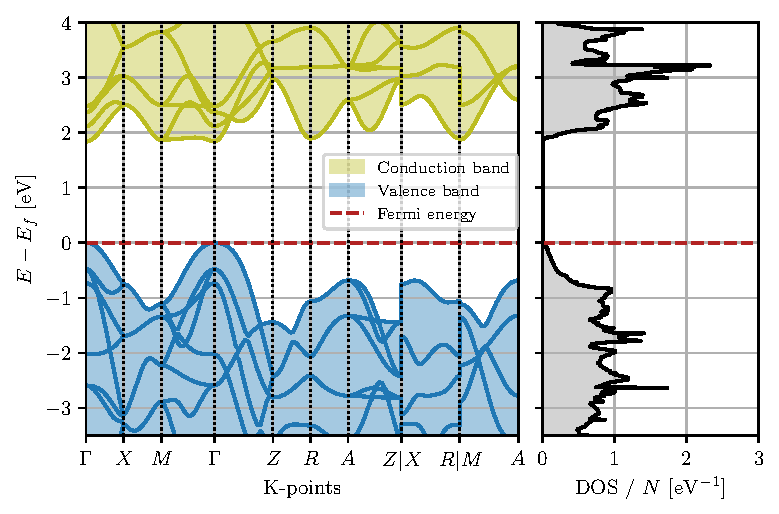
\includegraphics[width=\textwidth]{figures/unit_cell}
        \caption{Standard DFT}
        \label{fig:bands_unit_dft}
    \end{subfigure}
    \begin{subfigure}[t]{0.95\textwidth}
        \centering
        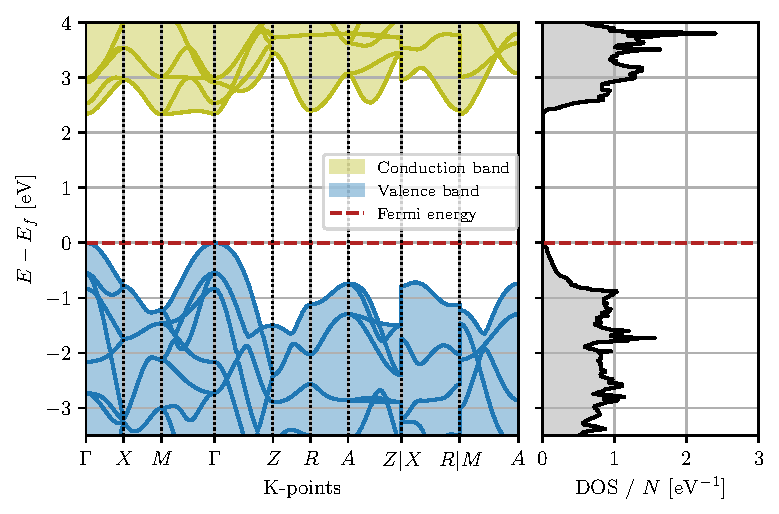
\includegraphics[width=\textwidth]{figures/unit_cell_u}
        \caption{DFT+U}
        \label{fig:bands_unit_dft+u}
    \end{subfigure}
    \caption{Band structure and DOS of the $\ce{TiO_2}$ rutile unit cell. The zero of the energy scale is set to the Fermi energy $E_f$. The DOS is divided by the total number of atoms $N = 6$.
        The direct ($\Gamma - \Gamma$) band gap in (a) is \SI{1.83}{eV}, whereas in (b) it is \SI{2.33}{eV}.}
    \label{fig:bands_unit}
\end{figure}

The localization of the electron with the vanadium atom at the center of the cell was successful. A new state with spin +$\mu_B$ was formed in the conduction band, ax expected for an atom with one extra electron. The magnetic moment of all the atoms was zero except for the vanadium one. The central vanadium had a magnetic moment of $\SI{1.093}{\mu_B}$. Substituting the vanadium atom with a titanium one, the extra electron remained localizes. This was confirmed by a magnetic moment on the central atom of \SI{0.930}{\mu_B} and an extra state in the valence band visible in the DOS. Finally, setting $U-J$ to \SI{3.9}{eV} also for the central titanium atom, the final polaron state was found. The magnetic moment on the central atom was \SI{0.787}{\mu_B} and a new state was created \SI{0.74}{eV} under the conduction band (in correspondence of the $\Gamma$ k-point).

The DOS and the band structure of the polaronic solution are reported in \cref{fig:polaron_bands}. From the picture the extra state is clearly visible both from the DOS and from the band structure. The Fermi energy is just above this new state. On the other hand, the delocalized solution is reported in \cref{fig:delocalized_bands}. The extra electron enters the conduction band, and the Fermi energy is shifted accordingly.

\begin{figure}
    \centering
    \begin{subfigure}[b]{\textwidth}
        \centering
        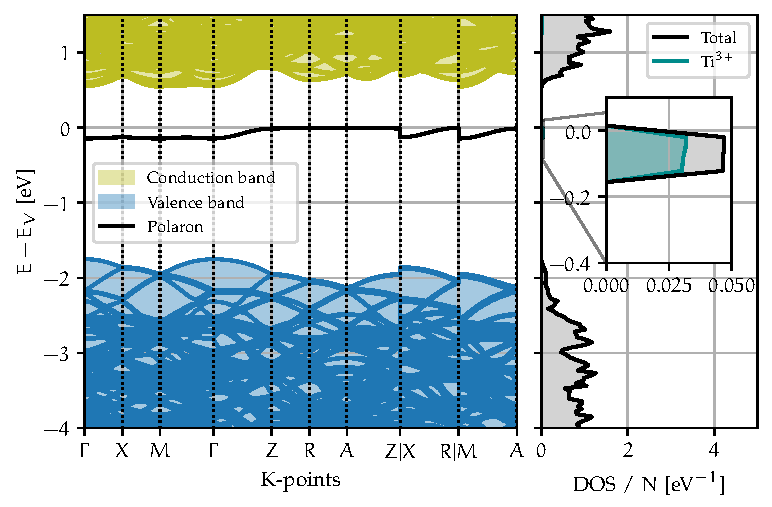
\includegraphics[width=\textwidth]{figures/polaron}
        \caption{Electron localized: polaron}
        \label{fig:polaron_bands}
    \end{subfigure}
    \hfill
    \begin{subfigure}[b]{\textwidth}
        \centering
        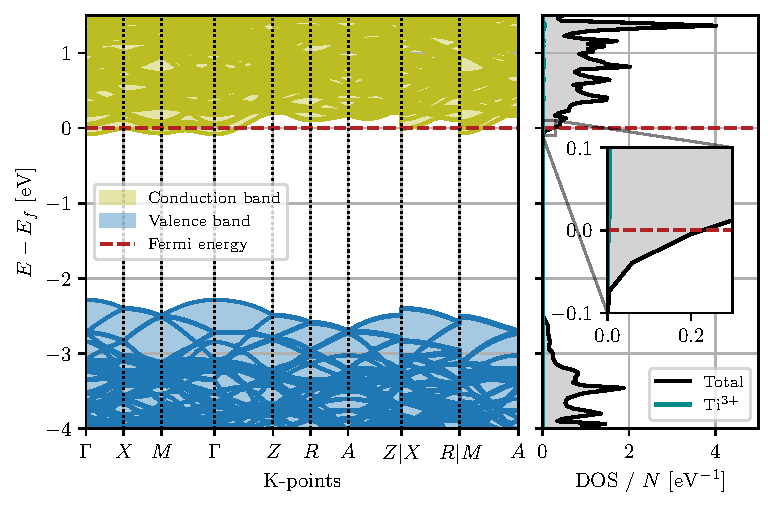
\includegraphics[width=\textwidth]{figures/deloc}
        \caption{Electron delocalized}
        \label{fig:delocalized_bands}
    \end{subfigure}
    \caption{Band structure and DOS of the $\ce{TiO_2}$ rutile supercell. The zero of the energy scale is set to the Fermi energy $E_f$. The DOS is divided by the total number of atoms $N = 162$. In (a) in addition to the total DOS, the partial DOS of the central atom - where the electron is localized - is reported as well.}
    \label{fig:bands_super}
\end{figure}

The isosurfaces of the charge densities of both solutions, projected on the band of the extra electron, are reported in \cref{fig:isosurfaces_supercell,fig:isosurfaces_center}. In the polaronic solution, the extra electron is localized on the central titanium atom, and the oxygen atoms around it are displaced by \SI{}{\angstrom}. Conversely, in the delocalized solution the electron is delocalized on all the atoms of the supercell.

\begin{figure}
    \centering
    \begin{subfigure}[b]{0.49\textwidth}
        \centering
        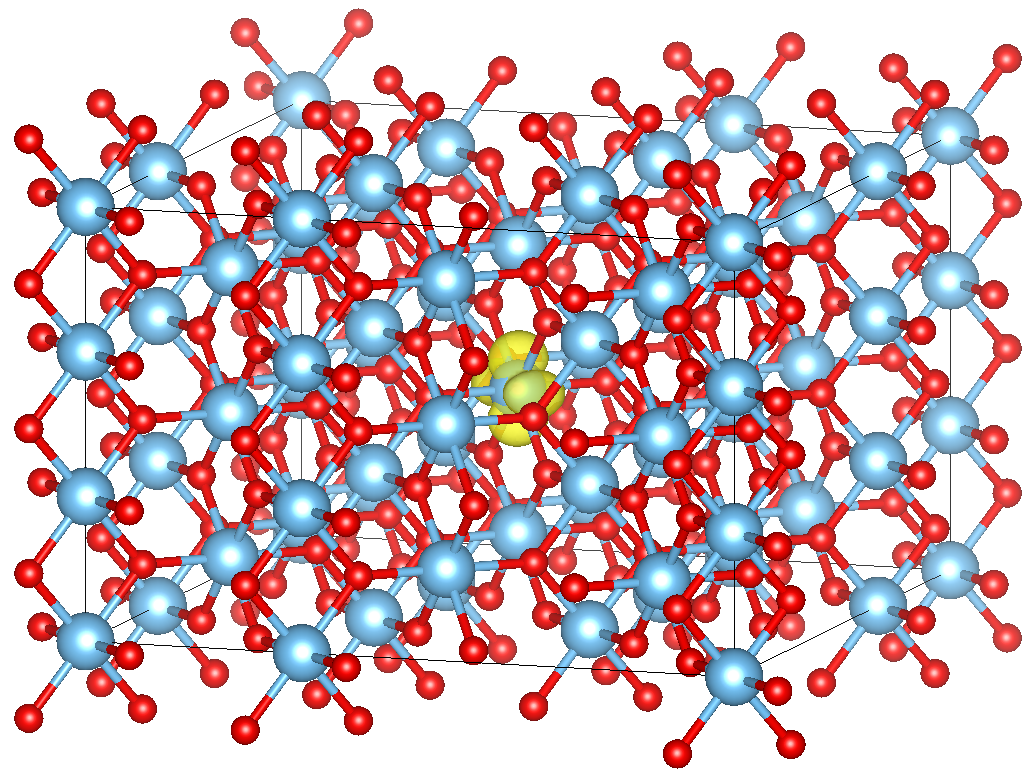
\includegraphics[width=\textwidth]{figures/PARCHG_polaron_super}
        \caption{Electron localized: polaron}
        \label{fig:polaron_iso}
    \end{subfigure}
    \hfill
    \begin{subfigure}[b]{0.49\textwidth}
        \centering
        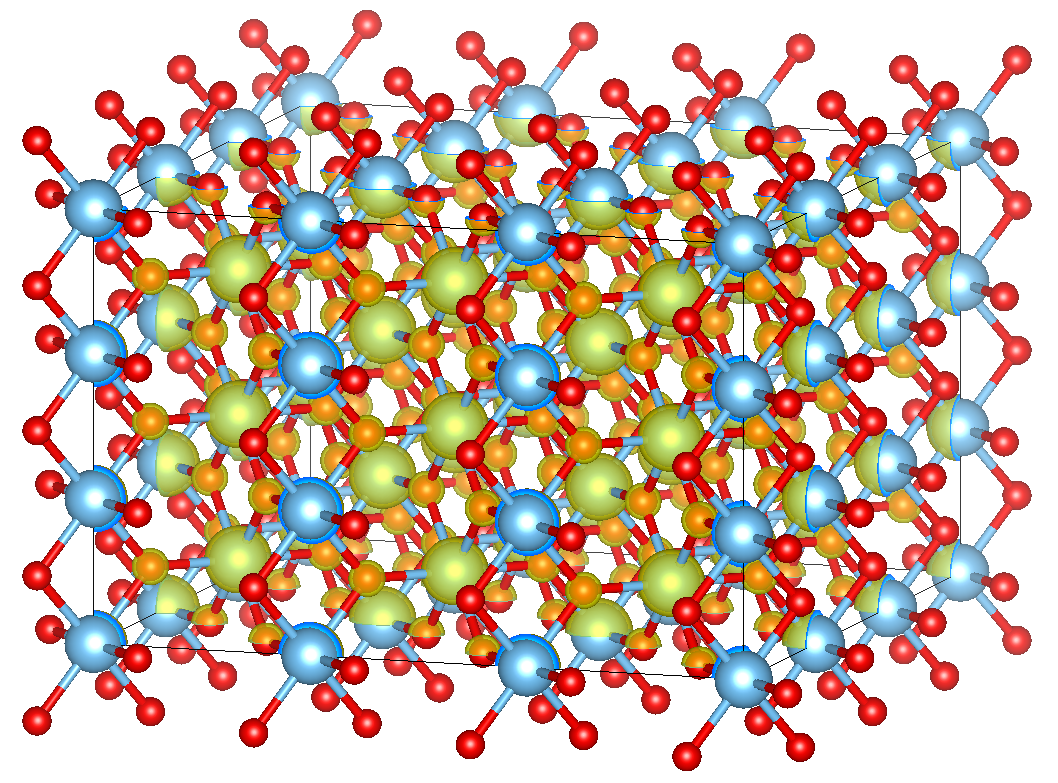
\includegraphics[width=\textwidth]{figures/PARCHG_delocalized_super}
        \caption{Electron delocalized}
        \label{fig:delocalized_iso}
    \end{subfigure}
    \caption{Supercell with the isosurface of the charge density projected on the extra-electron band. In (a) the extra electron is localized and forms a polaron, in (b) it is delocalized. The blue atoms are titanium atoms, whereas the red ones oxygen atoms.
    }
    \label{fig:isosurfaces_supercell}
\end{figure}

\begin{figure}
    \centering
    \begin{subfigure}[b]{0.49\textwidth}
        \centering
        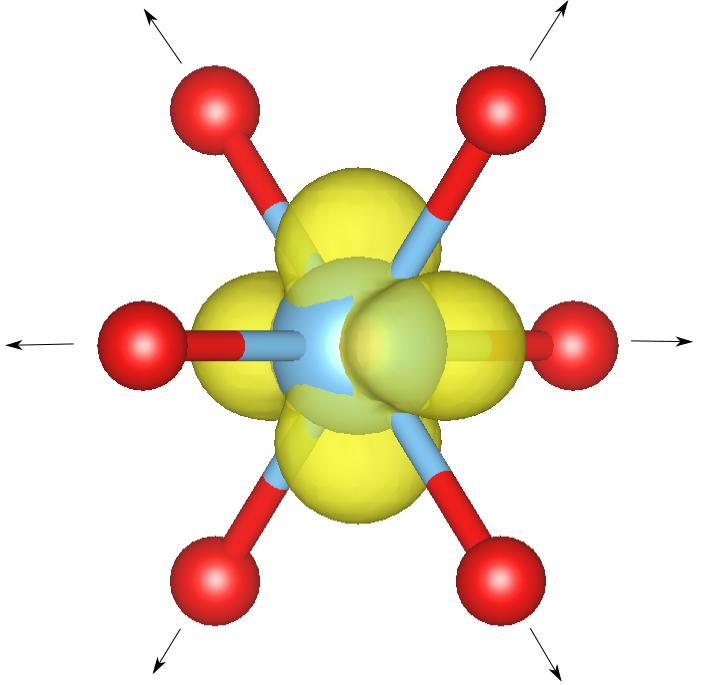
\includegraphics[width=\textwidth]{figures/PARCHG_polaron}
        \caption{Electron localized: polaron}
        \label{fig:polaron_iso}
    \end{subfigure}
    \hfill
    \begin{subfigure}[b]{0.49\textwidth}
        \centering
        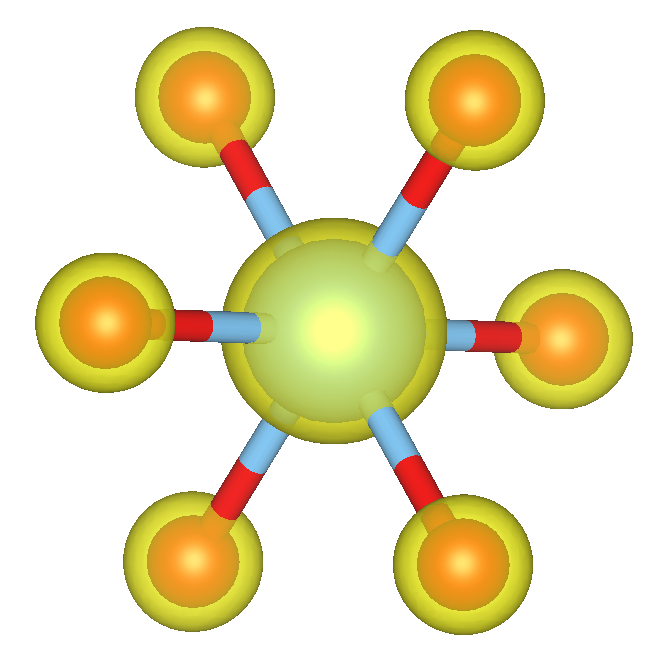
\includegraphics[width=\textwidth]{figures/PARCHG_delocalized}
        \caption{Electron delocalized}
        \label{fig:delocalized_iso}
    \end{subfigure}
    \caption{Isosurface of the charge density projected on the extra-electron band. In (a) the extra electron is localized and forms a polaron, in (b) it is delocalized. The blue atom is the central titanium atom, whereas the red ones are the nearest-neighbours oxygen atoms. In the polaronic solution the oxygen atoms are displaced by \SI{}{\angstrom} from their equilibrium positions.
    }
    \label{fig:isosurfaces_center}
\end{figure}
